% !TeX root = surprises.tex

\selectlanguage{hebrew}

\chapter{חלוקת זווית לשלושה חלקים}
\label{c.trisect}

לא ניתן לחלק זווית שרירותית לשלושה חלקים שווים באמצעות סרגל ומחוגה (להלן, בקיצור, לחלק זווית לשלושה). הסיבה היא שחלוקת זווית לשלושה דורשת בנייה של שורש שלישי, אבל עם  סרגל ומחוגה ניתן לבנות רק אורכים שמתקבלים מארבעת פעולות החשבון ושורש ריבועי. משפט זה הוכח ב-%
$1837$
על ידי
\L{Pierre Wantzel},
אולם חובבנים אינספור מנסים עד היום לחלק זווית לשלושה. הם בונים רק קירובים למרות שהם משוכנעים שהבניות נכונות. סעיף%
~\ref{s.trisect-approx}
מביא שתי בניות, מפתח את הנוסחאות לזוויות ומראה את השגיאות של הקירובים.

היוונים גילו שניתן לחלק זווית לשלושה אם משתמשים בכלים אחרים: הניאוסיס 
\L{(neusis)}
של
\L{Archimedes}
(סעיף%
~\ref{s.neusis})
והקוודרטריקס
\L{(quadratrix)}
של
\L{Hippias}
(סעיף%
~\ref{s.q}).
בסעיף%
~\ref{s.neusis-doubling}
נראה איך להכפיל קוביה באמצעות ניאוסיס.

שאר הפרק מביא הוכחה שלא ניתן לחלק זווית לשלושה. סעיף%
~\ref{s.trisect-constructible}
מאפיין מספרים בני-בנייה, סעיף%
~\ref{s.trisect-poly}
קושר מספרים בני-בנייה לשורשים של פולינומים, וסעיף%
~\ref{s.trisect-impossible}
משתמש בתיאוריה זו כדי להראות שלא ניתן לחלק זווית לשלושה או להכפיל קוביה.

%%%%%%%%%%%%%%%%%%%%%%%%%%%%%%%%%%%%%%%%%%%%%%%%%%%%%%%%%%%%


\section{קירובים לחלקת זווית לשלושה חלקים}\label{s.trisect-approx}

\subsection{הקירוב הראשון}\label{sub.trisect-approx1}

\noindent\textbf{בנייה:}

תהי 
$\theta=\angle AOB$
זווית שרירותית וללא הגבלת הכלליות נניח ש-%
$A,B$
נמצאות על מעגל היחידה שמרכזו 
$O$.
נבנה את חוצה הזוושית 
$\angle AOB$
ותהי 
$C$
נקודת החיתוך של חוצה הזווית עם מעגל היחידה. תהי
$D$
נקודת האמצע של
$\overline{OA}$
ותהי
$T$ 
נקודת האמצע של
$\overline{DC}$.
נסמן את הזווית
$\angle DOT$
על ידי
$\phi$
(איור%
~\ref{f.trisect-first-approx-1}).

\begin{figure}[tb]
\begin{center}
\begin{tikzpicture}[scale=.7]
\coordinate (O) at (0,0)
  node[left] {$O$}
  node[above right,xshift=14pt,yshift=16pt] {\sm{\theta/2}}
  node[right,xshift=19pt,yshift=5pt] {\sm{\theta/2}};
\coordinate (A) at (9cm,0);
\node[right] at (A) {$A$};
\coordinate (B) at (60:9);
\node[above] at (B) {$B$};
\draw (A) arc(0:60:9);
\draw (B) -- (O) -- (A);
\coordinate (C) at (30:9);
\node[right] at (C) {$C$};
\draw (O) -- node[above] {$1$} (C);
\coordinate (D) at (4.5,0);
\node[below] at (D) {$D$};
\coordinate (T) at ($(D)!.5!(C)$);
\draw (D) -- node[left] {$a$} (T) -- node[left] {$a$} (C);
\node[right] at (T) {$T$};
\draw (O) -- (T);
\draw (	1,0) arc (0:30:1);
\draw (30:.8) arc (30:60:.8);
\draw (2,0) arc (0:20:2);
\node[above right] at (2.1,0.1) {\sm{\phi}}; 

\draw[<->] (0,-1) -- node[fill=white] {\sm{1/2}} +(4.5,0);
\draw[<->] (4.5,-1) -- node[fill=white] {\sm{1/2}} +(4.5,0);
\end{tikzpicture}
\end{center}
\caption{קירוב ראשון ($1$)}\label{f.trisect-first-approx-1}
\end{figure}

\begin{theorem}
\[\tan\phi =\frac{2\sin(\theta/2)}{1+2\cos(\theta/2)}\,.\]
\end{theorem}

\begin{proof}
איור%
~\ref{f.trisect-first-approx-2}
נלקח מאיור
~\ref{f.trisect-first-approx-1}
עם סימונים נוספים.

יהי
$\overline{CF}$
האנך ל-%
$\overline{OA}$
שחוצה את
$\overline{OA}$
ב-%
$F$.
$\overline{CF}=\sin (\theta/2)$
ו-%
$\overline{OF}=\cos(\theta/2)$
כי
$\overline{OC}=1$.
יהי
$\overline{TE}$
האנך ל-%
$\overline{OA}$
שחוצה את
$\overline{OA}$
ב-%
$E$.

$T$
היא נקודת האמצע של
$\overline{DC}$
ולכן
$\overline{DT}=\overline{TC}=a$.
אבל
$\overline{FT}$
הוא תיכון ליתר של משולש ישר-זווית, כך ש-%
$\overline{FT}=a$
ומכאן ש-%
$\triangle DTF$
שווי-שוקיים. 
$\overline{TE}$
הוא גם תיכון וגם גובה ל-%
$\overline{DF}$.
מהאיור קל לראות ש:
\[
\overline{OE}=\frac{1}{2} + \frac{1}{2}\left(\cos \frac{\theta}{2}-\frac{1}{2}\right)\,.
\]
\begin{figure}[tb]
\begin{center}
\begin{tikzpicture}[scale=1]
\coordinate (O) at (0,0)
  node[left] {$O$}
  node[right,xshift=26pt,yshift=5pt] {\sm{\theta/2}};
\coordinate (A) at (9cm,0);
\node[right] at (A) {$A$};
\draw (O) -- (A);
\coordinate (C) at (30:9);
\node[right] at (C) {$C$};
\draw (O) -- node[above] {\sm{1}} (C);
\coordinate (D) at (4.5,0);
\node[below] at (D) {$D$};
\coordinate (T) at ($(D)!.5!(C)$);
\draw (D) -- node[left] {\sm{a}} (T) -- node[left] {\sm{a}} (C);
\node[right] at (T) {$T$};
\draw (O) -- (T);
\draw (	1,0) arc (0:30:1);
\draw (2,0) arc (0:20:2);
\node[above right] at (1.9,0.1) {\sm{\phi}}; 

\coordinate (E) at (T |- A);
\draw[thick,dashed] (T) -- node[right] {\sm{h}}
  (E) node[below] {$E$};
\draw[rotate=90] (E) rectangle +(7pt,7pt);

\coordinate (F) at (C |- A);
\draw[thick,dashed] (C) --
  node[right] {\sm{\sin (\theta/2)}} (F) node[below] {$F$};
\draw[rotate=90] (F) rectangle +(7pt,7pt);

\draw[thick,dashed] (T) -- node[right] {\sm{a}} (F);

\draw[<->] ($(O)+(0,-1)$) --
  node[fill=white] {\sm{1/2}} +(4.5,0);
\draw[<->] ($(O)+(0,-1.8)$) --
  node[fill=white] {\sm{\cos (\theta/2)}} ($(F)+(0,-1.8)$);
\draw[<->] ($(D)+(0,-2.6)$) --
  node[fill=white] {\sm{\left(\cos (\theta/2)\!-\! (1/2)\right)}} 
  ($(F)+(0,-2.6)$);
\draw[<->] ($(O)+(0,-3.4)$) --
  node[fill=white] {\sm{(1/2)+(1/2)\left(\cos (\theta/2)\! -\! (1/2)\right)}} 
  ($(E)+(0,-3.4)$);
\end{tikzpicture}
\end{center}
\caption{קירוב ראשון ($2$)}\label{f.trisect-first-approx-2}
\end{figure}
נחשב את האורך
$2a=\overline{CD}$
באמצעות משפט פיתגורס ב-%
$\triangle DCF$:
\begin{eqn}
(2a)^2 &=&  \left(\cos \frac{\theta}{2}-\frac{1}{2}\right)^2+\sin^2\frac{\theta}{2}\,.
\end{eqn}
ניתן לחשב את אורכו של
$h=\overline{TE}$
ממשפט פיתגורס ב-%
$\triangle DTE$:
\begin{eqn}
a^2 &=& h^2 + \left[\frac{1}{2}\left(\cos \frac{\theta}{2}-\frac{1}{2}\right)\right]^2\\
h^2&=&\frac{1}{4}\left(\cos \frac{\theta}{2}-\frac{1}{2}\right)^2+\frac{1}{4}\sin^2\frac{\theta}{2}-\left[\frac{1}{2}\left(\cos \frac{\theta}{2}-\frac{1}{2}\right)\right]^2=
\frac{1}{4}\sin^2\frac{\theta}{2}\\
h&=&\frac{1}{2}\sin\frac{\theta}{2}\\
\tan\phi &=&\frac{h}{\overline{OE}}=\displaystyle\frac{\displaystyle\frac{1}{2}\sin\frac{\theta}{2}}{\displaystyle\frac{1}{2}+\frac{1}{2}\left(\cos \frac{\theta}{2}\! -\! \frac{1}{2}\right)}
=\frac{\displaystyle2\sin\frac{\theta}{2}}{\displaystyle 1+2\cos\frac{\theta}{2}}\,.
\end{eqn}
\end{proof}

זה קירוב לחלוקת זווית לשלושה חלקים
$\phi=\theta/3$.
עבור
$\theta=60^\circ$:
\[
\tan^{-1}\left(\frac{2\sin 30^\circ}{1+2\cos 30^\circ}\right)=
\tan^{-1}0.366\approx 20.1^\circ\approx 20^\circ\,.
\]
טבלה%
~\ref{t.trisect-first}
מראה את השגיעות עבור טווח של זוויות חדות. השגיעה קטנה יחסית עבור זוויות קטנות אבל עולה עד
$1\%$
עבור
$85^\circ$.

\begin{table}[t]
\[
%
\begin{array}{r@{\hspace{5mm}}r@{\hspace{5mm}}r@{\hspace{5mm}}r@{\hspace{5mm}}r}
\hline
\noalign{\smallskip}
\theta ({}^\circ) & \theta/3 ({}^\circ)& \tan^{-1} \phi ({}^\circ) & \mathrm{Error} ({}^\circ) & \mathrm{Error (\%)}\\\hline
\noalign{\smallskip}
  5 &    1.667 &    1.667  &     0.000 &    0.004 \\
 10 &    3.333 &    3.334  &     0.000 &    0.014 \\
 15 &    5.000 &    5.002  &     0.002 &    0.032 \\
 20 &    6.667 &    6.670  &     0.004 &    0.057 \\
 25 &    8.333 &    8.341  &     0.007 &    0.088 \\
 30 &   10.000 &   10.013  &     0.013 &    0.128 \\
 35 &   11.667 &   11.687  &     0.020 &    0.174 \\
 40 &   13.333 &   13.364  &     0.030 &    0.228 \\
 45 &   15.000 &   15.043  &     0.043 &    0.289 \\
 50 &   16.667 &   16.726  &     0.060 &    0.358 \\
 55 &   18.333 &   18.413  &     0.080 &    0.435 \\
 60 &   20.000 &   20.104  &     0.104 &    0.520 \\
 65 &   21.667 &   21.799  &     0.133 &    0.612 \\
 70 &   23.333 &   23.500  &     0.166 &    0.713 \\
 75 &   25.000 &   25.206  &     0.206 &    0.823 \\
 80 &   26.667 &   26.918  &     0.251 &    0.941 \\
 85 &   28.333 &   28.636  &     0.303 &    1.068 \\
 \noalign{\smallskip}
 \hline
 \end{array}
\]
\caption{שגיאות בקירוב הראשון}\label{t.trisect-first}
\end{table}

%%%%%%%%%%%%%%%%%%%%%%%%%%%%%%%%%%%%%%%%%%%%%%%%55

\subsection{הקירוב השני}

\noindent\textbf{בנייה:}

תהי
$\theta=\angle AOB$
זווית שרורותית ונניח ללא הגבלת הכלליות ש-%
$A,B$
נמצאות על מעגל יחידה שמרכזו
$O$.
נבנה מעגל שהרדיוס שלו
$1/3$
שמרכזו
$O$
ותהי
$D$
נקודת החיתוך שלו עם
$\overline{OA}$.
נבנה את חוצה הזווית
$\angle AOB$
ותהי
$C$
נקודת החיתוך שלו עם המעגל שהרדיוס שלו
$1/3$.
נבנה את המיתר
$\overline{CD}$
והמיתרים
$\overline{AE}=\overline{ET}=\overline{CD}$.
בגלל שמיתרים שווים נשענים על ידי זוויות מרכזיות שוות,
$\angle TOE=\angle EOA=\phi$
(איור~\ref{f.trisect-second-approx}).

\begin{figure}[tb]
\begin{center}
\begin{tikzpicture}[scale=.75]
\coordinate (O) at (0,0)
  node[left] {$O$}
  node[above right,xshift=10pt,yshift=12pt] {\sm{\theta/2}};
\coordinate (A) at (9cm,0);
\node[right] at (A) {$A$};
\coordinate (B) at (60:9);
\node[above] at (B) {$B$};
\draw (A) arc(0:60:9);
\draw (B) -- (O) -- (A);
\coordinate (D) at (3,0);
\node[below] at (D) {$D$};
\draw[name path=third] (D) arc(0:60:3);
\coordinate (C) at (30:3);
\node[right] at (C) {$C$};
\draw (O) -- node[above,near end] {\sm{1/3}} (C);
\draw[thick] (D) -- (C);
\coordinate (E) at (10:9);
\node[right] at (E) {$E$};
\draw[thick] (A) -- node[right] {\sm{1/3}} (E);
\coordinate (T) at (20:9);
\node[right] at (T) {$T$};
\draw[thick] (E) -- node[right] {\sm{1/3}} (T);
\draw (O) -- node[above,near end] {\sm{1}} (T);

\draw (	1,0) arc (0:30:1);
\draw (30:.8) arc (30:60:.8);
\draw (4,0) arc (0:20:4);
\node at (4.2,0.35) {\sm{\phi}}; 
\node at (4.1,1.1) {\sm{\phi}}; 

\draw[dashed] (O) --
  node[fill=white,inner sep=0pt,very near start,
       xshift=9pt,yshift=1pt] {\sm{\theta/2}} 
  node[fill=white,near end] {$1$} (E);

\draw[<->] (3,-.8) -- node[fill=white] {\sm{2/3}} +(6,0);
\draw[<->] (0,-.8) -- node[fill=white] {\sm{1/3}} +(3,0);
\end{tikzpicture}
\end{center}
\caption{הקירוב השני}
\label{f.trisect-second-approx}
\end{figure}

\begin{theorem}
\[
\cos\phi=1 - \frac{1}{9}(1-\cos(\theta/2))=1 - \frac{2}{9}\sin^2(\theta/4)\,.
\]
\end{theorem}

\begin{proof}
לפי חוק הקוסינוסים ב-%
$\triangle DOC$:
\[
\overline{CD}= \left(\frac{1}{3}\right)^2+\left(\frac{1}{3}\right)^2-2\left(\frac{1}{3}\right)\left(\frac{1}{3}\right)\cos (\theta/2)=\frac{2}{9}(1-\cos(\theta/2))\,.
\]
לפי חוק הקוסינוסים ב-%
$\triangle EOA$:
\[
\overline{AE} = 1^2+1^2-2\cdot 1\cdot 1\cdot \cos \phi=2(1-\cos \phi)\,.
\]
נשווה שת שתי הביטויים עבור
$\overline{CD}=\overline{AE}$,
נפשט ונקבל:
\[
\cos \phi = 1 - \frac{1}{9}(1-\cos(\theta/2))\,.
\]
בגלל ש-%
$\cos 2\alpha= \cos^2 \alpha-\sin^2\alpha=1-2\sin^2\alpha$
ולכן
$1-\cos 2\alpha=2\sin^2\alpha$,
נקבל את הביטוי החלופי:
\[
\cos \phi = 1 - \frac{2}{9}\sin^2(\theta/4)\,.
\]
\end{proof}

זה קירוב לחלוקת זווית לשלושה חלקים
$2\phi=\theta/3$.
עבור
$\theta=60^\circ$:
\[
2\cos^{-1}\left(1 - \frac{1}{9}(1-\cos 30^\circ)\right)\approx 19.8^\circ\approx 20^\circ\,.
\]
טבלה%
~\ref{t.trisect-second-approx}
מראה את השגיאות עבור טווח של זוויות חדות. בנייה זו הרבה בפחות מדוייק מהבנייה בסעיף%
~\ref{sub.trisect-approx1}.

\begin{table}[t]
\[
\begin{array}{r@{\hspace{5mm}}r@{\hspace{5mm}}r@{\hspace{5mm}}r@{\hspace{5mm}}r}
\hline
\noalign{\smallskip}
\theta ({}^\circ) & \theta/3 ({}^\circ)& \cos^{-1} 2\phi ({}^\circ) & \mathrm{Error} ({}^\circ) & \mathrm{Error (\%)}\\
\noalign{\smallskip}\hline\noalign{\smallskip}
  5 &    1.667 &    1.667  &     0.000 &    0.007 \\
 10 &    3.333 &    3.332  &     0.001 &    0.028 \\
 15 &    5.000 &    4.997  &     0.003 &    0.063 \\
 20 &    6.667 &    6.659  &     0.008 &    0.113 \\
 25 &    8.333 &    8.319  &     0.015 &    0.176 \\
 30 &   10.000 &    9.975  &     0.025 &    0.254 \\
 35 &   11.667 &   11.626  &     0.040 &    0.346 \\
 40 &   13.333 &   13.273  &     0.060 &    0.451 \\
 45 &   15.000 &   14.914  &     0.086 &    0.571 \\
 50 &   16.667 &   16.549  &     0.118 &    0.705 \\
 55 &   18.333 &   18.177  &     0.156 &    0.853 \\
 60 &   20.000 &   19.797  &     0.203 &    1.015 \\
 65 &   21.667 &   21.408  &     0.258 &    1.192 \\
 70 &   23.333 &   23.011  &     0.322 &    1.382 \\
 75 &   25.000 &   24.603  &     0.397 &    1.586 \\
 80 &   26.667 &   26.185  &     0.481 &    1.805 \\
 85 &   28.333 &   27.756  &     0.577 &    2.038 \\
 \noalign{\smallskip}
 \hline
 \end{array}
\]
\caption{שגיאות בקירוב השני}
\label{t.trisect-second-approx}
\end{table}

%%%%%%%%%%%%%%%%%%%%%%%%%%%%%%%%%%%%%%%%%%%%%%%%%%%%%%%%%%%%%

\section{חלוקת זווית לשלושה באמצעות ניאוסיס}
\label{s.neusis}

השימוש במילה "סרגל" מטעה כי הכוונה היא למקל ישר ללא כל סימן, שהפעולה היחידה שניתן לעשות איתו היא למתוח קו ישר בין שתי נקודות. 
\L{Archimedes}
הראה שניתן להשתמש
\textbf{בניאוסיס},
מקל עם שני סימנים בלבד, כדי לחלק זווית לשלושה. נגדיר את המרחק בין שני הסימנים כ-%
$1$
(איור%
~\ref{f.neusis}).
\begin{figure}[tb]
\begin{center}
\begin{tikzpicture}[scale=3.5]
\draw (-1,1.05) rectangle +(3.2,.1);
\draw[thick] (1.89,1.05) -- +(0,.1);
\draw[thick] (.73,1.05) -- +(0,.1);
\draw[<->] (.73,1.25) -- node[fill=white] {$1$} (1.89,1.25);
\end{tikzpicture}
\end{center}
\caption{ניאוסיס}\label{f.neusis}
\end{figure}

\textbf{בנייה:}
תהי 
$\alpha$
זווית שרירותית
$\angle ABE$
בתוך מעגל יחידה שמרכזו
$B$
שהוא המרחק בין הסינמים על הניאוסיס. נמשיך את קטע הקו
$\overline{EB}$
מחוץ למעגל. שנשים את הניאוסיס על הנקודה
$A$
ונזיז אותו עד שהוא חותך את הקו בנקודה 
$D$
ואת המעגל בנקודה
$C$.
נכוון את הניאוסיס כך שהאורכו של
$\overline{CD}$
יהיה
$1$.
נבנה את הקו
$\overline{AD}$.
נסמן
$\angle CDB=\beta$
(איור%
~\ref{f.trisect-neusis-1}).
\begin{figure}[tb]
\begin{center}
\begin{tikzpicture}[scale=2.5]
\coordinate (origin) at (0,0) node[below] {$B$} ;
\draw[name path=circle] (origin) circle [radius=1];
\draw (origin) node[above left,xshift=-4pt] {$\alpha$} -- (120:1) coordinate (a) node[below,xshift=-2pt] {$A$} ;
\draw (-1,0) -- (2.2,0);
\path[name path=ad] (a) -- (0,0 -| 2,0) coordinate (d) node[below] {$D$} ;
\path[name intersections={of=circle and ad,by={c,a1}}];
\fill (origin) circle [radius=.5pt];
\fill (a) circle [radius=.5pt];
\fill (c) circle [radius=.5pt] node [below,xshift=-4pt] {$C$};
\fill (d) circle [radius=.5pt];
\fill (-1,0) circle [radius=.5pt] node [left] {$E$};
\begin{scope}[rotate=-19,yshift=-11.25pt]
\draw (-1,1.05) rectangle +(3.2,.1);
\draw[thick] (1.89,1.05) -- +(0,.1);
\draw[thick] (.76,1.05) -- +(0,.1);
\draw[<->] (.73,1.25) -- node[fill=white] {$1$} (1.89,1.25);
\end{scope}
\end{tikzpicture}
\end{center}
\selectlanguage{hebrew}
\caption{חלוקת זווית לשלושה חלקים באמצעות ניאוסיס (1)}\label{f.trisect-neusis-1}
\end{figure}

\begin{figure}[tb]
\begin{center}
\begin{tikzpicture}[scale=2.5]
\coordinate (origin) at (0,0) node[below] {$B$} ;
\draw[name path=circle] (origin) circle [radius=1];
\draw (origin) node[above left,xshift=-4pt] {$\alpha$} node[above,xshift=4pt,yshift=2pt] {$\delta$} node[above right,xshift=44pt,yshift=-2pt] {$\beta$} -- node[fill=white] {$1$} (120:1) coordinate (a) node[above left] {$A$} ;
\draw (-1,0) -- (2.2,0);
\draw[name path=ad] (a) node[below right,xshift=8pt,yshift=-6pt] {$\gamma$} -- (0,0 -| 2,0) coordinate (d) node[left,xshift=-50pt,yshift=7pt] {$\beta$} node[above right] {$D$} ;
\path[name intersections={of=circle and ad,by={c,a1}}];
\draw (origin) -- node[fill=white] {$1$}(c) node[above right] {$C$} node[left,xshift=-12pt] {$\gamma$} node[below,xshift=-2pt,yshift=-2pt] {$\epsilon$};
\fill (origin) circle [radius=.5pt];
\fill (a) circle [radius=.5pt];
\fill (d) circle [radius=.5pt];
\fill (c) circle [radius=.5pt];
\fill (-1,0) circle [radius=.5pt];
\path (c) -- node[fill=white] {$1$} (d);
\end{tikzpicture}
\selectlanguage{hebrew}
\caption{חלוקת זווית לשלושה חלקים באמצעות ניאוסיס (2)}\label{f.trisect-neusis-2}
\end{center}
\end{figure}

\begin{theorem}
$\beta=\alpha/3$.
\end{theorem}
\begin{proof}
נבנה את
$\overline{BC}$
ונסמן את הזוויות ואת קטעי הקו כפי שרשום באיור%
~\ref{f.trisect-neusis-2}.
$\triangle ABC$, $\triangle BCD$
הם משולשים שווי-שוקיים:
$\overline{AB}=\overline{BC}$
הם רדיוסים של אותו מעגל ו-%
$\overline{BC}=\overline{CD}$
לפי הבנייה באמצעות הניאוסיס. סכום הזוויות של משולש שווה ל-%
$180^\circ$
כמו גם סכום הזוויות המשלימות, לכן 
\begin{eqn}
\epsilon &=& 180^\circ - 2\beta\\
\gamma &=& 180^\circ - \epsilon = 2\beta\\
\delta &=& 180^\circ - 2\gamma = 180^\circ - 4\beta\\
\alpha &=& 180^\circ - \delta - \beta = 4\beta -\beta =3\beta\,.
\end{eqn}
\end{proof}

%%%%%%%%%%%%%%%%%%%%%%%%%%%%%%%%%%%%%%%%%%%%%%%%%%%%%%%%%%%%%

\section{הכפלת קוביה באמצעות ניאוסיס}\label{s.neusis-doubling}

נתונה קוביה 
$C$
יש לבנות קוביה עם נפח כפול. אם הנפח של 
$C$
הוא
$V$
הצלעות שלה באורך
$\sqrt[3]{V}$.
אורך צלעות הקוביה עם נפח כפול הוא
$\sqrt[3]{2 V}=\sqrt[3]{2}\cdot\sqrt[3]{V}$, 
ולכן אם ניתן לבנות
$\sqrt[3]{2}$
נוכל להכפיל קוביה.

\noindent\textbf{בנייה:}
נבנה משולש שווה-צלעות
$\triangle ABC$
ונמשיך את
$\overline{CA}$
עם קטע קו באורך אחד עד ל-%
$D$.
נבנה קרנות שממשיכות את
$\overline{AB}$
ו-%
$\overline{DB}$.
נניח את הניאוסיס על הנקודה 
$C$
ונזיז אותו עד שסימן אחד שלו נמצאת על הקרן
$\overline{AB}$
ב-%
$P$
והסימן השני על הקרן
$\overline{DB}$
ב-%
$Q$.
נסמן
$\overline{CQ}=x$
ו-%
$\overline{BP}=y$
(איור%
~\ref{f.double-neusis}).

\begin{figure}[tb]
\begin{center}
\begin{tikzpicture}[scale=.7]
\clip (-.7,-.4) rectangle +(11.2,6.5);
\coordinate (D) at (0,0) node[left] {$D$};
\draw (D) -- ++(60:6) coordinate (C) node[above] {$C$};
\coordinate (A) at (60:3);
\node[left] at (A) {$A$};
\draw (A) -- ++(3,0) coordinate (B) -- (C);
\node[below right] at (B) {$B$};
\path[name path=DQ] (D) -- ($(D)!1.7!(B)$);
\path[name path=AP] (A) -- ($(A)!3!(B)$);
% 3*(1+\sqrt[3]{2}) = 6.78
\path[name path=CP] (C) circle (6.78cm);
\path[name intersections={of=CP and AP,by={P}}];
\draw[name path=CP] (C) -- (P);
\path[name intersections={of=CP and DQ,by={Q}}];
\node[above] at (Q) {$Q$};
\node[right] at (P) {$P$};
\draw (D) -- (Q);
\draw (B) -- (P);
\path (D) -- node[left] {$1$} (A) -- node[left] {$1$} (C) --
  node[right] {$1$} (B) -- node[below] {$1$} (A);
\path (C) -- node[above] {$x$} (Q) -- node[above] {$1$} (P) -- 
  node[below] {$y$} (B);
\end{tikzpicture}
\end{center}
\caption{הכפלת הקוביה עם ניאוסיס}\label{f.double-neusis}
\end{figure}

\begin{theorem}
$x=\sqrt[3]{2}$.
\end{theorem}

\begin{proof}
$\triangle ABC$
שווה-צלעות ולכן
$\cos \angle CAP=\cos 60^\circ=\frac{1}{2}$
ולפי חוק הקוסינוס ב-%
$\triangle APC$:
\begin{eqnlabels}
\overline{CP}&=&\overline{AC}^2+\overline{AP}^2-2\cdot \overline{AC}\cdot\overline{AP}\cos 60^\circ\\
(x+1)^2&=&1^2+(y+1)^2-2\cdot 1\cdot (y+1)\cdot \frac{1}{2}\\
x^2+2x&=&y^2+y\label{eq.eq-cube-double}\,.
\end{eqnlabels}
לפי חוק
\L{Menelaus}
(משפט%
~\ref{thm.menelaus}):
\[
\displaystyle\frac{\overline{AB}}{\overline{BP}}\cdot
\displaystyle\frac{\overline{PQ}}{\overline{QC}}\cdot
\displaystyle\frac{\overline{CD}}{\overline{DA}}=1\,.
\]
ולכן:
\begin{eqnlabels}
\displaystyle\frac{1}{y}\cdot
\displaystyle\frac{1}{x}\cdot
\displaystyle\frac{2}{1}&=&1\\
xy&=&2\,.\label{eq.menelaus-xy2}
\end{eqnlabels}
נציב משוואה%
~\ref{eq.menelaus-xy2}
במשוואה%
~\ref{eq.eq-cube-double}
ונקבל:
\begin{eqn}
x^2+2x&=&\frac{4}{x^2}+\frac{2}{x}\\
x^4+2x^3&=&4+2x\\
x^3(x+2)&=&2(x+2)\\
%x^3&=&2\\
x&=&\sqrt[3]{2}\,.
\end{eqn}
\end{proof}

%%%%%%%%%%%%%%%%%%%%%%%%%%%%%%%%%%%%%%%%%%%%%%%%%%%%%%%%%%%%%

\section{חלוקת זווית לשלושה באמצעות
קוודרטריקס%
}\label{s.q}

יהי
$\overline{ABCD}$
ריבוע. יהי
$l_1$
קטע קו המונח תחילה ב-%
$\overline{DC}$
ויהי
$l_2$
קטע קו המונח תחילה ב-%
$\overline{AD}$. 
נזיז את
$l_1$
במהירות ליניארית קבועה עד שהוא מגיע ל-%
$\overline{AB}$
ונסובב את
$l_2$
במהירות סיבובית קבועה מסביב ל-%
$A$
עד שגם הוא מגיע ל-%
$\overline{AB}$.
נניח שהם מגיעים ל-%
$\overline{AB}$
ביחד. למשל, אם
$l_2$
מסתובב ב-%
$1^\circ$
לשנייה ואורך הריבוע הוא
$9$
ס"מ,
$l_1$
חייב בזוז ב-%
$0.1$
שנייה/ס"מ. העקומה הנוצרת על ידי נקודת החיתוך 
$P$
נקראת
\L{\textbf{quadratrix curve}}
או פשוט 
\textbf{קוודרטריקס}
\L{\textbf{(quadratrix)}}
(\ref{f.trisect-quad-curve}). 
ההגדרה מיוחסת למתמטיקאי
\L{Hippias}\index{Hippias}.

\ref{f.trisect-quad-compass}
מראה
\textbf{מחוגת קוודרטריקס}
המורכב משני סרגלים (ללא סימנים) הזזים כפי שמתואר לעיל. מפרק המאלץ אותם לנוע ביחד ומייצר עקומה.

\begin{figure}[tb]
\begin{center}
\begin{subfigure}{.45\textwidth}
\begin{tikzpicture}[scale=.6,domain=.03:1.555,samples=100]
\draw (.1,.2)
  node[below left,xshift=-8pt] {$A$} -- 
  (7.8,.2) 
  node[below right] {$B$} -- 
  (8,7.8) 
  node[above right] {$C$} -- 
  (.1,7.8) node[above left,xshift=-8pt] {$D$} -- 
  cycle;
\draw[thick,dashed,name path=arm] (.1,.2) -- node[right,very near end] {$l_2$} (59.6:7.9);
\draw[thick,dashed,name path=horiz] (.1,5) -- node[above,near end] {$l_1$} +(7.8,0);
\path[name intersections={of=arm and horiz,by={A}}];
\node[above left,xshift=-2pt] at (A) {$P$};
\vertex{A};
\draw[thick] plot (4.6*.637*\x,{12.2*.637*\x*cot(\x r)});
\end{tikzpicture}
\selectlanguage{hebrew}
\caption{עקומת קוודראטריס}\label{f.trisect-quad-curve}
\end{subfigure}
\hspace{2em}
\begin{subfigure}{.45\textwidth}
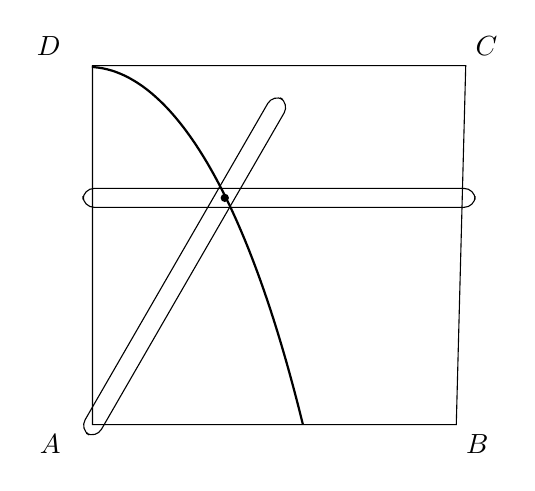
\begin{tikzpicture}[scale=.6,domain=.03:1.555,samples=100]
\draw (.1,.2) node[below left,xshift=-8pt] {$A$} -- (7.8,.2) node[below right] {$B$} -- (8,7.8) node[above right] {$C$} -- (.1,7.8) node[above left,xshift=-8pt] {$D$} -- cycle;
\draw[rounded corners,rotate=60] (0,-.2) rectangle (8.2,.2);
\draw[rounded corners] (-.1,4.8) rectangle (8.2,5.2);
\fill (2.9,5) circle [radius=2.5pt];
\draw[thick] plot (4.6*.637*\x,{12.2*.637*\x*cot(\x r)});
\end{tikzpicture}
\selectlanguage{hebrew}
\caption{מחוגה קוודראטריקס}\label{f.trisect-quad-compass}
\end{subfigure}
\end{center}
\end{figure}

ניתן להשתמש בקוודראטריקס כדי לחלק זוויות לשלושה.

\textbf{בנייה:}
תהי
$\angle CDP_1=\alpha$
זווית שרירותית כאשר 
$P_1$
היא נקודת החיתוך של הקו המגדיר את הזווית
$\alpha$
יחסית ל-%
$\overline{DC}$
והקוודראטריקס. נבנה קו דרך 
$P_1$
מקביל ל-%
$\overline{DC}$
ונסמן ב-%
$E$
את החיתוך שלו עם
$\overline{AD}$.
נסמן את טקע הקו 
$\overline{DE}$
ב-%
$t$
ונחלק אותו לשלושה חלקים שווים (סעיף%
~\ref{s.trisect-constructible})
עדי לקבל את הנקודה
$F$
שהיא
$t/3$
מ-%
$\overline{DC}$.
תהי
$P_2$
נקודת החיתוך של קו מ-%
$F$
מקביל ל-%
$\overline{DC}$
והקוודראטריקס, ונסמן ב-%
$\theta$
את הזווית בין
$\overline{DC}$
ן-%
$\overline{DP_2}$
(איור%
~\ref{f.trisect-quad-trisect}).
\begin{theorem}
$\theta=\alpha/3$.
\end{theorem}
\begin{proof}
קואורדינטת ה-%
$y$
של
$E$
היא
$1-t$,
ולכן ל-%
$F$
קואורדינטת ה-%
$y$
שווה ל-%
$1-(t/3)$.
המהירות הליניארית הקבועה של הסרגל האופקי ביחס קבוע למהירות הזוויתית הקבועה של הסרגל המסתובב, ולכן
$\theta/\alpha = (t/3)/t$
ו-%
$\theta = \alpha/3$.
\end{proof}

\begin{figure}[tb]
\begin{center}
\begin{tikzpicture}[scale=.8,domain=.03:1.562,samples=100]
\draw (.1,7.8) coordinate (start) node[above left] {$D$} node[below right,xshift=32pt] {$\theta$} -- (.1,.2) node[below left] {$A$} -- (8,.1) node[below right] {$B$} -- (8,7.8) node[above right] {$C$} -- cycle;
\draw[name path=curve,thick] plot (4.6*.637*\x,{12.2*.637*\x*cot(\x r)});
\path[name path=twenty] (start) -- +(-35:9);
\path[name path=sixty] (start) -- +(-50:9);
\path[name path=xaxis] (.1,.2) -- (8,.1);
\path[name intersections={of=twenty and curve,by={x1,tri}}];
\draw (start) -- (tri);
\fill (tri) circle [radius=2pt] node[right] {$P_2$};
\path[name intersections={of=sixty and curve,by={x2,angle}}];
\fill (angle) circle [radius=2pt] node[right] {$P_1$};
\draw (start) -- (angle);
\path[name intersections={of=xaxis and curve,by=x}];
\fill (x) circle [radius=2pt];
%\path (.1,.2) -- node[below] {$2/\pi$} (x);
\draw[dashed] (tri) -- (tri -| .1,.2) coordinate (t3);
\fill (t3) circle [radius=2pt] node[left] {$F$};
\draw[dashed] (angle) -- (angle -| .1,.2) coordinate (t);
\fill (t) circle [radius=2pt] node[left] {$E$};
\draw[<->] (-1.2,7.8) -- node[fill=white] {$t/3$} (-1.2,7.8 |- t3);
\draw[<->] (-.6,7.8) -- node[fill=white] {$t$} (-.6,7.8 |- t);
\draw[<->] (-.6,7.8 |- t) -- node[fill=white] {$1-t$} (-.6,.2);
\draw (3.5,7.8) arc[start angle=0,delta angle=-49,radius=3.5];
\draw (1,7.8) arc[start angle=0,delta angle=-32,radius=1];
\node at (3.3,6) {$\alpha$}; 
\end{tikzpicture}
\end{center}
\selectlanguage{hebrew}
\caption{חלוקת זווית לשלושה באמצעות קוודרטריקס}\label{f.trisect-quad-trisect}
\end{figure}

%%%%%%%%%%%%%%%%%%%%%%%%%%%%%%%%%%%%%%%%%%%%%%%%%%

\section{מספרים בני-בנייה}\label{s.trisect-constructible}

יהי 
$l$
קטע קו שאורכו מוגדר כ-%
$1$.
\begin{definition}
מספר
$a$
הוא
\textbf{בן-בנייה \L{(constructible)}}
אם ורק אם ניתן לבנות באמצעות סרגל ומחוגה קטע קו באורך
$a$
כאשר מתחילים עם
$l$.
\end{definition}
נתון קטע קו
$l=\overline{AB}$,
נבנה קו המכיל את
$\overline{AB}$
ונשתמש במחוגה כדי למוצא נקודה
$C$
על הקו במרחק
$1$
מ-%
$B$.
מכאן שאורכו של
$\overline{AC}$
הוא
$2$
ולכן המספר
$2$
בן-בנייה. ניתן לבנות קטע קו
$\overline{BD}$
באורך
$1$
ניצב ל-%
$\overline{AB}$
ב-%
$B$.
היתר של המשולש
$\triangle ABD$
הוא באורך
$\sqrt{2}$
ולכן המספר
$\sqrt{2}$
בן-בנייה.

\begin{theorem}\label{thm.trisect-constructible}
מספר הוא
\textbf{בן-בנייה}
אם ורק אם הוא ערכו שביטוי שנבנה ממספרים שלמים, ארבעת פעולת החשבון
$\{+,-,\times,/\}$
ופעולת השורש הריבועי
$\surd$.
\end{theorem}

\begin{figure}[tb]
\begin{center}
\begin{tikzpicture}[scale=.8]
\coordinate (P) at (0,0);
\coordinate (Q) at (5,0);
\coordinate (T) at (3,0);
\coordinate (U) at (7,0);
\vertex{P};
\vertex{Q};
\draw (P) -- (Q);
\node[above] at (P) {$P$};
\node[above left] at (Q) {$Q$};
\node[above left] at (U) {$U$};
\node[above right] at (T) {$T$};
\draw (5,0) -- (8,0);
\draw (5,0) circle[radius=2cm];
\draw (5,0) -- node[left] {$b$} ++(60:2cm);
\coordinate (R) at (9,-1);
\coordinate (S) at ($(9,-1) + (20:2cm)$);
\vertex{R};
\vertex{S};
\draw (R) node[above] {$R$} --
  node[below right] {$b$} (S)
  node[above] {$S$};
\draw[<->] (0,-.5) -- node[fill=white] {$a$} (5,-.5);
\draw[<->] (0,-1) -- node[fill=white] {$a-b$} (3,-1);
\draw[<->] (0,-1.5) -- node[fill=white] {$a+b$} (7,-1.5);
\end{tikzpicture}
\end{center}
\selectlanguage{hebrew}
\caption{בניית חיבור וחיסור}\label{f.trisect-add-subtract}
\end{figure}

\begin{proof}
תחילה נראה שניתן לבנות את המספרים המתקבלים מהפעולות.

\noindent\textbf{חיבור וחיסור:}
נתונים קטעי קו
$\overline{PQ}=a$
ו-%
$\overline{RS}=b$,
נבנה מעגל שמרכזו
$Q$
עם רדיוס
$b$
(איור%
~\ref{f.trisect-add-subtract}).
נמשיך את
$\overline{PQ}$
עד שהוא חותך את המעגל ב-%
$U$.
אזי
$\overline{PTQU}$
הוא קטע קו כאשר
$\overline{PT}=a-b$
ו-%
 $\overline{PU}=a+b$.

\smallskip

\noindent\textbf{כפל:}
לפי משולשים דומים ב%
\ref{f.trisect-multiplication},
$(1/b)=(a/\overline{OA})$
ולכן
$\overline{OA}=ab$.

\smallskip

\noindent\textbf{חילוק:}
לפי משולשים דומים ב%
\ref{f.trisect-division},
$(1/b)=(\overline{OD}/a)$
ולכן
$\overline{OD}=(a/b)$.

\begin{figure}[tb]
\begin{center}
\begin{subfigure}{.45\textwidth}
\begin{tikzpicture}[scale=.8]
\draw[name path=horz] (0,0) coordinate (o) -- (7,0);
\node[left] at (o) {$O$};
\coordinate (a) at (6,0);
\node[below]  at (a) {$A$};
\draw (o) -- (30:5.5);
\coordinate (c) at (30:3);
\coordinate (b) at (30:5);
\node[above] at (c) {$C$};
\node[above] at (b) {$B$};
\draw (a) -- (b);
\path[name path=par] (c) -- +($(a)-(b)$);
\path[name intersections={of=par and horz,by=d}];
\node[below] at (d) {$D$};
\draw (c) -- (d);
\draw[<->] (-.4,.5) -- node[fill=white] {$b$} +(30:5.2);
\path (o) -- node[above] {$1$} (c);
\draw[<->] (0,-.8) -- node[fill=white] {$ab$} +(6,0);
\path (o) -- node[below] {$a$} (d);
\end{tikzpicture}
\selectlanguage{hebrew}
\caption{בניית כפל}\label{f.trisect-multiplication}
\end{subfigure}
\hspace{2em}
\begin{subfigure}[b]{.45\textwidth}
\begin{tikzpicture}[scale=.8]
\draw[name path=horz] (0,0) coordinate (o) -- (7,0);
\node[left] at (o) {$O$};
\coordinate (a) at (6,0);
\node[below]  at (a) {$A$};
\draw (o) -- (30:5.5);
\coordinate (c) at (30:3);
\coordinate (b) at (30:5);
\node[above] at (c) {$C$};
\node[above] at (b) {$B$};
\draw (a) -- (b);
\path[name path=par] (c) -- +($(a)-(b)$);
\path[name intersections={of=par and horz,by=d}];
\node[below] at (d) {$D$};
\draw (c) -- (d);
\draw[<->] (-.4,.5) -- node[fill=white] {$b$} +(30:5.2);
\path (o) -- node[above] {$1$} (c);
\draw[<->] (0,-.8) -- node[fill=white] {$a$} +(6,0);
\path (o) -- node[below] {$a/b$} (d);
\end{tikzpicture}
\selectlanguage{hebrew}
\caption{בניית חילוק}\label{f.trisect-division}
\end{subfigure}
\end{center}
\end{figure}

\smallskip

\noindent\textbf{שורש ריבועי:}
נתון קטע קן
$\overline{BC}=a$,
נבנה
$\overline{AB} =1+a$
ומחצית המגעל שקוטרו
$\overline{AB}$.
נבנה ניצב ב-%
$C$
ונסמן ב-%
$D$
את החיתוך של הניצב והמעגל (איור%
~\ref{f.trisect-square-root}). $\angle ADB$
הוא משולש יישר-זווית כי הוא נשען על קוטר. לפי משולשים דומים
$(h/1)=(a/h)$
ולכן
$h^2=a$
ו-%
$h=\sqrt{a}$.

\begin{figure}[tb]
\begin{center}
\begin{tikzpicture}[scale=1]
\draw[name path=horz] (0,0) coordinate (a) -- (6,0);
\node[left] at (a) {$A$};
\coordinate (b) at (6,0);
\node[below] at (b) {$B$};
\draw[name path=circle] (b) arc(0:180:3);
\path[name path=perp] (2,0) -- +(0,3.2);
\coordinate (c) at (2,0);
\node[below] at (c) {$C$};
\path[name intersections={of=circle and perp,by=d}];
\node[above] at (d) {$D$};
\draw (c) -- node[right] {$h$} (d);
\path (a) -- node[below] {$1$} (c) -- node[below] {$a$} (b);
\draw (c) rectangle +(6pt,6pt);
\draw (a) -- (d) -- (b);
\draw[rotate=-125] (d) rectangle +(6pt,6pt);
\node[above right,xshift=4pt] at (a) {$\alpha$};
\node[above left,xshift=-12pt] at (b) {$90^\circ\!-\!\alpha$};
\node[below right,yshift=-8pt] at (d) {$\alpha$};
\node[below left,xshift=0pt,yshift=-18pt] at (d) {$90^\circ\!-\!\alpha$};
\end{tikzpicture}
\end{center}
\caption{בניית שורש}
\label{f.trisect-square-root}
\end{figure}

\medskip

כדי להוכיח את הכיוון השני של המשפט, עלינו לקבוע איזו מספרים ניתן לבנות באמצעות סרגל ומחוגה. קיימות שלוש בניות:%
\footnote{%
למען הבהירות נדגים אותן על ערכים מסויימים במקום להשתמש במשוואות הכלליות.}
\begin{enumerate}
\item
שני קווים נחתכים בנקודה 
(\ref{f.constructible-two-lines}).
ניתן לחשב את הקואורדינטות של נקודה החיתוך מהמשוואות של שני הקווים
$y=x$
ו-%
$y=4x-2$.
נקודת החיתוך היא
$P= (2/3, 2/3)$.
\item
קו חותך מעגל באפס, אחת או שתי נקודות 
(\ref{f.constructible-line-circle}).
ניתן לחשב את הקואורדינטות של נקודות החיתוך מהמשוואות של הקו 
$y=x$
והמעגל
$x^2+y^2=4$.
נקודות החיתוך היא
$P=(\sqrt{2}, \sqrt{2})$ and $Q=(-\sqrt{2}, -\sqrt{2})$.
\item
שני מעגלים נחתכים באפס, אחת או שתי נקודה (איור%
~\ref{f.constructible-two-circles}).
ניתן לחשב את הקואורדינטות של נקודות החיתוך מהמשוואות של שני המעגלים:
\begin{eqn}
(x-1)^2+y^2&=&4\\
(x+1)^2+y^2&=&4\,.
\end{eqn}
נקודות החיתוך הן
$P=(0,\sqrt{2}),Q=(0,-\sqrt{2})$.
\end{enumerate}\vspace{-5ex}
\end{proof}

\begin{figure}[tb]
\begin{center}
\begin{subfigure}{.4\textwidth}
\begin{tikzpicture}[scale=.66]
\draw[step=10mm,white!50!black,very thin] (-4,-4) grid (4,4);
\draw[thick] (-4,0) -- (4,0);
\draw[thick] (0,-4) -- (0,4);
\coordinate (O) at (0,0);
\foreach \x in {-3,...,4}
  \node at (\x-.2,-.3) {\sm{\x}};
\foreach \y in {-3,...,-1}
  \node at (-.4,\y-.3) {\sm{\y}};
\foreach \y in {1,...,4}
  \node at (-.3,\y-.3) {\sm{\y}};
\draw[name path=eq1] (-4,-4) -- (4,4);
\draw[name path=eq2] (-.5,-4) -- (1.5,4);
\path[name intersections={of=eq1 and eq2,by={P}}];
\node[right] at (P) {$P$};
\end{tikzpicture}
\caption{נקודת החיתוך של שני קווים}\label{f.constructible-two-lines}
\end{subfigure}
\hspace{3em}
\begin{subfigure}[b]{.4\textwidth}
\begin{tikzpicture}[scale=.66]
\coordinate (O) at (0,0);
\draw[step=10mm,white!50!black,very thin] (-4,-4) grid (4,4);
\draw[thick] (-4,0) -- (4,0);
\draw[thick] (0,-4) -- (0,4);
\foreach \x in {-3,...,4}
  \node at (\x-.2,-.3) {\sm{\x}};
\foreach \y in {-3,...,-1}
  \node at (-.4,\y-.3) {\sm{\y}};
\foreach \y in {1,...,4}
  \node at (-.3,\y-.3) {\sm{\y}};
\coordinate (A) at (2,0);
\node[draw,circle through=(A),name path=circle] at (0,0) {};
\draw[name path=eq1] (-4,-4) -- (4,4);
\path[name intersections={of=eq1 and circle,by={P,Q}}];
\node[right] at (P) {$P$};
\node[left] at (Q) {$Q$};
\end{tikzpicture}
\caption{נקודות החיתוך של קו ומעגל}\label{f.constructible-line-circle}
\end{subfigure}
\end{center}
\end{figure}

\begin{figure}[tb]
\begin{center}
\begin{tikzpicture}[scale=.66]
\coordinate (O) at (0,0);
\draw[step=10mm,white!50!black,very thin] (-4,-4) grid (4,4);
\draw[thick] (-4,0) -- (4,0);
\draw[thick] (0,-4) -- (0,4);
\foreach \x in {-3,...,4}
  \node at (\x-.2,-.3) {\sm{\x}};
\foreach \y in {-3,...,-1}
  \node at (-.4,\y-.3) {\sm{\y}};
\foreach \y in {1,...,4}
  \node at (-.3,\y-.3) {\sm{\y}};
\coordinate (A) at (3,0);
\node[draw,circle through=(A),name path=circle1] at (1,0) {};
\coordinate (B) at (-3,0);
\node[draw,circle through=(B),name path=circle2] at (-1,0) {};
\path[name intersections={of=circle1 and circle2,by={P,Q}}];
\node[right,xshift=6pt,yshift=-2pt] at (P) {$P$};
\node[right,xshift=6pt,yshift=2pt] at (Q) {$Q$};
\end{tikzpicture}
\caption{נקודות החיתוך של שני מעגלים}\label{f.constructible-two-circles}
\end{center}
\end{figure}

%%%%%%%%%%%%%%%%%%%%%%%%%%%%%%%%%%%%%%%%%%%%%%%%%%%%

\section{מספרים בני-בנייה כשורשים של פולינומים}\label{s.trisect-poly}

כדי לראות שמספר איננו בן-בנייה יש להוכיח שלא ניתן לבטא אותו רק עם המספרים השלמים והפעולות
$\{+,-,\times,/,\surd\}$.
נראה שמספרים בני-בנייה הם השורשים של קבוצה מסויימת של פולינומים ואז נוכיח שחלוקת זווית לשלושה חלקים והכפלת קוביה מחייבות לבנות שורשים של פולינומים שאינם איברים בקבוצה. היום מוכיחים את התוצאות הללו באמצעות תורת השדות מאלגברה, אבל פה אביא הוכחה שמשתמשת במתמטיקה בסיסית. ההוכחה מבוססת על ההגדרה שלהלן.
\begin{definition}
\textbf{העומק}
של ביטוי שמורכב ממספרים שלמים ומהפעולות
$\{+,-,\times,/,\surd\}$
הוא רמת הקינון המירבית של שורש ריבועי.
\end{definition}
\begin{example}
בביטוי שלהלן:
\[
\sqrt{17+3\sqrt{17} - \sqrt{34-2\sqrt{17}}
  -2\sqrt{34+2\sqrt{17}} }\,,
\]
העומק הוא
$3$
כי בצד הימין של הביטוי נמצא
$\sqrt{17}$
שמקונן תוך
$\sqrt{34+2\sqrt{17}}$
שבעצמו מקונן בתוך
$\sqrt{17+\cdots-\cdots-2\sqrt{34+2\sqrt{17}}}$.
\end{example}

\begin{theorem}
ניתן לבטא ביטוי בעומק
$n$
כ-%
$a+b\sqrt{c}$
כאשר
$a,b,c$
הם ביטויים בעמוק
$n-1$
לכל היותר.
\end{theorem}
\begin{proof}
חישובים פשוטים מראים שהתוצאות של הביטויים 
$(a_1+b_1\sqrt{c})\,\mathit{op}\,(a_2+b_2\sqrt{c})$
עבור הפעולות
$\mathit{op}=\{+,-,\times\}$
הן ביטויים
$a+b\sqrt{c}$
בעומק
$n-1$.
עבור חילוק החישוב מעט יותר מסובך:
\begin{eqn}
\frac{a_1+b_1\sqrt{c}}{a_2+b_2\sqrt{c}}&=&
\frac{(a_1+b_1\sqrt{c})(a_2-b_2\sqrt{c_2})}{(a_2+b_2\sqrt{c})(a_2-b_2\sqrt{c})}\\
&=&\frac{a_1a_2-b_1b_2c}{a_2^2-b_2^2c}+\frac{a_2b_1-a_1b_2}{a_2^2-b_2^2c}\sqrt{c}\,,
\end{eqn}
שהוא מהצורה 
$a+b\sqrt{c}$
ובעומק
$n\!-\!1$.
לבסוף, השורש של ביטוי בעומק
$n\!-\!1$
הוא בעומק
$n$.
\end{proof}

\begin{theorem}\label{thm.trisect.conjugate}
יהי
$p(x)$
פולינום ממעלה שלוש מונית עם מקדמים רציונליים:
\[
p(x)=x^3+a_2x^2+a_1x+a_0\,,
\]
ויהי
$r=a+b\sqrt{c}$
שורש של
$p(x)$
בעל עומק
\textbf{מינימלי}
$n$,
כאשר 
$a,b,c$
מם בעומק
$n-1$
לכל היותר. אזי
$r'=a-b\sqrt{c}$
הוא שורש של
$p(x)$
ו-%
$r\neq r'$.
\end{theorem}

\begin{proof}
נחשב
$p(r)$
שווה ל-%
$0$
כי
$r$
הוא שורש:
\[
\renewcommand{\arraystretch}{1.3}
\begin{array}{lcr}
(a+b\sqrt{c})^3+a_2(a+b\sqrt{c})^2+a_1(a+b\sqrt{c})+a_0&=\\
(a^3+3a^2b\sqrt{c}+3ab^2c+b^3c\sqrt{c})\\
\quad+\,a_2(a^2+2ab\sqrt{c}+b^2c) +a_1(a+b\sqrt{c}) +a_0&=\\
(a^3+3ab^2c+a_2a^2+a_2b^2c+a_1a+a_0)\\
\quad+\,(3a^2b+b^3c+2a_2ab+a_1b)\sqrt{c}&=\\
d+e\sqrt{c}&=&0\,,
\end{array}
\]
כאשר
$d,e$
הם ביטויים בעומק
$n-1$
שמורכבים ממקדמים רציונליים ו-%
$a,b,c$.
אזי
$\sqrt{c}=-d/e$
כך שניתן לבטא את
$a+b\sqrt{c}$
כביטוי בעומק
$n-1$,
סתירה להנחה ש-%
$a+b\sqrt{c}$
הוא מעומק מינימלי. בגלל ש-%
$\sqrt{c}\neq 0$
ועומק
$n$,
כדי ש-%
$d+e\sqrt{c}$
יהיה שווה לאפס חייב להתקיים
$d=e=0$.

מה עם
$r'=a-b\sqrt{c}$?
אם נעיין בחישוב למעלה נראה ש-%
$p(r')=d-e\sqrt{c}=0+0\cdot\sqrt{c}=0$
כך שגם
$r'$
הוא שורש של
$p$.
אם
$r= r'$
אזי
$0=r-r'=2b\sqrt{c}$
שהוא נכון רק אם
$b=0$
ואז העומק של
$r,r'$
יהיה 
$n-1$,
שוב בסתירה להנחה.
\end{proof}                                

\begin{theorem}
אם לפולינום ממעלה שלוש עם מקדמים רציונליים:
\[p(x)=x^3+a_2x^2+a_1x+a_0\]
אין שורשים רציונליים, אז אף אחד מהשורשים שלו אינו בן-בנייה.
\end{theorem}

\begin{proof}
לפי המשפט הבסיסי של אלגברה (משפט%
~\ref{thm.fundamental}) 
ל-%
$p(x)$
שלושה שורשים
$r_1,r_2,r_3$.
יהי
$r_1=a+b\sqrt{c}$
השורש עם העומק המינימלי
$n$.
לפי ההנחה שאין שורשים רציונליים,
$n\geq 1$,
ולכן
$b\neq 0$
ו-%
$c\neq 0$.
לפי משפט%
~\ref{thm.trisect.conjugate}, $r_2=a-b\sqrt{c}$ 
הוא גם שורש. נבצע את הכפל שלהלן:
\begin{eqnlabels}
(x-r_1)(x-r_2)(x-r_3)&=&x^3 -(r_1+r_2+r_3)x^2\\
&&\quad\; +\, (r_1r_2+r_1r_3+r_2r_3)x + r_1r_2r_3\label{eq.viete3}\\
a_2&=&-(r_1+r_2+r_3)\\
r_3&=&-(a_2+r_1+r_2)\,.
\end{eqnlabels}
אבל
$a_2$
הוא רציונלי ולכן גם:
\[r_3=-a_2-(r_1+r_2)=-a_2-2a\,,\]
רציונלי בסתירה להנחה.
\end{proof}

%%%%%%%%%%%%%%%%%%%%%%%%%%%%%%%%%%%%%%%%%%%%%%%%%%%%

\section{אי-אפשר לחלק זווית לשלושה חלקים ולהכפיל קוביה}\label{s.trisect-impossible}

\begin{theorem}\label{thm.trisect.cube-root-irrational}
$\sqrt[3]{2}$
אינו מספר רציונלי.
\end{theorem}
\begin{proof}
נניח ש-%
$\sqrt[3]{2}$
רציונלי ושווה ל-%
$p/q$
כאשר
$p,q$
מספרים שלמים ללא גורמים משותפים פרט ל-%
$\pm 1$.
אזי:
\begin{eqn}
(p/q)^3&=&(\sqrt[3]{2})^3\\
p^3&=&2q^3\,,
\end{eqn}
ולכן ניתן לחלק את
$p$
ב-%
$2$,
כלומר,
$p=2r$.
נמשיך:
\begin{eqn}
8r^3&=&2q^3\\
q^3&=&4r^3\,,
\end{eqn}
כך שניתן לחלק גם את
$q$
ב-%
$2$,
סתירה להנחה של-%
$p,q$
אין גורם משותף.
\end{proof}

\begin{theorem}
ל-%
$x^3-2$
אין שורשים רציונליים, ולכן לא ניתן להכפיל קוביה עם סרגל ומחוגה.
\end{theorem}
\begin{proof}
אחד מהשורשים הוא
$\sqrt[3]{2}$
שהוא לא רציונלי (משפט%
~\ref{thm.trisect.cube-root-irrational}).
השורשים האחרים הם השורשים של הפולינום הריבועית
$x^2+\sqrt[3]{2}x+(\sqrt[3]{2})^2$
שמתקבל כאשר מחלקים את
$x^3-2$
ב-%
$x-\sqrt[3]{2}$.
קל לבדוק שהשורשים לא רציונליים (למעשה, הם אפילו לא ממשיים).
\end{proof}

\begin{theorem}
לא ניתן לחלוק זווית שרירותית לשלושה עם סרגל ומחוגה.
\end{theorem}
\begin{proof}
מספיק להוכיח שיש זווית אחת שלא ניתנת לחלוקה. ננסה לחלק את
$60^\circ$
לשלושה חלקים כדי לקבל
$20^\circ$.
לפי משפט%
~\ref{thm.triple-angle}:
\begin{eqn}
\cos 3\alpha&=&4\cos^3\alpha -3\cos\alpha\\
\cos 60^\circ&=&4\cos^3 20^\circ -3\cos 20^\circ\,.
\end{eqn}
נסמן
$x=\cos 20^\circ$
ונסמן
$y=2x$.
מ-%
$\cos 60^\circ=1/2$
מתקבל:
\begin{eqn}
4x^3 -3x-\frac{1}{2} &=& 0\\
8x^3-6x-1&=&0\\
y^3-3y-1&=&0\,.
\end{eqn}
כדי להוכיח שלפולינום
$y^3-3y-1$
 אין שורשים רציונליים, נניח ש-%
$y=a/b$
הוא שורש רציונלי כאשר ל-%
$a,b$
אין גורמים משותפים פרט ל-%
$\pm 1$.
אזי:
\begin{eqnlabels}
(a/b)^3-3(a/b)-1&=&0\\
a^3-3ab^2&=&b^3\\
a(a-3b^2)&=&b^3\label{eq.trisect1}\\
a^3&=&b(b^2+3ab)\label{eq.trisect2}\,.
\end{eqnlabels}
לפי משוואה%
~\ref{eq.trisect1}, 
ניתן לחלק את
$b$
ב-%
$a$,
ולפי משוואה%
~\ref{eq.trisect2},
ניתן לחלק את
$a$
ב-%
$b$.
זה אפשרי רק אם
$a=b=\pm 1$ 
ו-%
$a/b=\pm 1$.
ניתן לבדוק בחישוב ש-%
$y=a/b=1$
ו-%
$y=a/b=-1$
אינם שורשים של הפולינום.
\end{proof}

דרך אחרת להוכיח שהבעיות אינן אפשריות היא להשתמש במשפט שלהלן (ללא הוכחה):
\begin{theorem}\label{thm.factor}
אם לפולינום עם מקדמים שלמים (שהמקדם הראשון הוא אחד(
$p(x)=x^n+a_{n-1}x^{n-1}+\cdots+a_0$
יש שורשים רציונליים, אזי יש לו שורשים שלמים.
\end{theorem}
כדי להראות שלא ניתן להכפיל את קוביה עלינו לראות שלפולינום:
\[
x^3-2=(x-r_2)(x-r_1)(x-r_0)
\]
אין שורשים שלמים. בגלל ש-%
$r_0r_1r_2=-2$
כל השורשים חייבים לחלק את
$2$,
כך שהשורשים השלמים האפשריים הם
$\pm 1, \pm 2$.
חישוב קצר מראה שאף אחד מהם אינו שורש.

כדי לראות שלא ניתן לחלק זווית לשלושה חלקים עלינו לראות שלפולינוים
$y^3-3y-1$
אין שורשים שלמים. שורש שלם חייב לחלק את
$-1$
אבל לא
$1$
ולא
$-1$
הם שורשים.

%%%%%%%%%%%%%%%%%%%%%%%%%%%%%%%%%%%%%%%%%%%%%%%%%%%%

\subsection*{מה ההפתעה?}

\L{Underwood Dudley}
ערך חקירה רחבה על מי שהוא כינה "תמהונים" שמבזבזים שנים של חייהם בניסיון להוכיח שניתן לחלק זוויות לשלושה. לא רק שהם מוליכים את עצמם שלל, אבל, גרוע מזה, הם חושבים שלמציאת בנייה חשיבות. כמובן, שבנייה היא חסרת שימוש מעשי כי עם כלים כגון הניאוסיס והקוודרטיקס ניתן למצוא בנייה מדוייקת. המספר העצום של הבניות הללו מפתיע כי רבים מהם מתוחכמות ומשיגים קירובים טובים. חישוב הנוסחאות של הבניות הגיאומטריות הוא תרגיל מצויין בטריגונומטריה.

מפתיע גם שההוכחות שלא ניתן לבצע את הבניות הללו משתמשות רק באלגברה ומבוססות על תכונות של שורשים של פולינומים.

%%%%%%%%%%%%%%%%%%%%%%%%%%%%%%%%%%%%%%%%%%%%%%%%%%%%

\subsection*{מקודות}

\L{Wikipedia} \cite{wiki:tri, wiki:neu, wiki:quad}
הוא מקור טוב למידע על בניות. שני הקירובים לחלוקת זווית לשלושה חלקים הם מ-%
\cite[עמודים
67-68, 95-96]{dudley-budget}.
הקירוב השני מיוחס לפילוסוף הנודע
\L{Thomas Hobbes}.
חלוקת זווית לשלושה באמצעות קוודראטיקס מבוסס על
\cite[עמודים~48-49]{martin}
ו-%
\cite[עמודים 6-7]{dudley-budget}.
הכפלת הקוביה באמצעות ניואסיס נלקחה מ-%
 \cite{dorrie2}.

אפשר למצוא הצגה מוקפדת של מספרים בני-בנייה בכל ספר לימוד לאלגברה מודרנית כגון
\cite{fraleigh},
שכולל הוכחה של המקרה הכללי של משפט%
~\ref{thm.trisect-constructible}
בסעיף~$32$. משפט%
~\ref{thm.factor}
הוא משפט%
~$23.11$
של
\cite{fraleigh}.
הוכחה נגישה יחסית של ההוכחה של 
\L{Wantzel}
נמצא ב-%
\cite{suzuki}.
ההצגה שלי של מספרים בני-בנייה מבוססת על ההצגות ב-%
\cite[פרק~\L{III}]{courant}
ו-%
\cite{laugwitz}.
